\documentclass[tikz,border=5pt]{standalone}
\usepackage{verbatim}
\usetikzlibrary{shadings,intersections}

\begin{document}
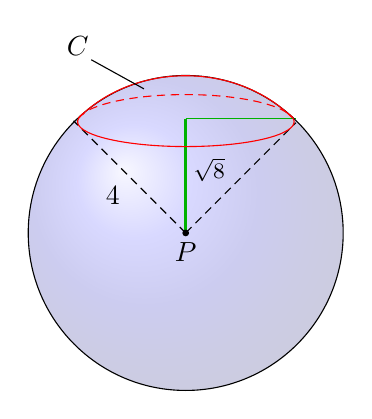
\begin{tikzpicture}

 \coordinate (O) at (0,0);

  % ball background color
  \shade[ball color = blue, opacity = 0.2] (0,0) circle [radius = 2cm];

	\draw [very thick, black!30!green] (0, 0) -- (0, 1.45) ;
	\draw [ black!30!green] (0, 1.45) -- (1.4, 1.45);

  % cone
  \begin{scope}
    \def\rx{0.71}% horizontal radius of the ellipse
    \def\ry{0.15}% vertical radius of the ellipse
    \def\z{0.725}% distance from center of ellipse to origin

    \path [name path = ellipse]    (0,\z) ellipse ({\rx} and {\ry});
    \path [name path = horizontal] (-\rx,\z-\ry*\ry/\z)
                                -- (\rx,\z-\ry*\ry/\z);
    \path [name intersections = {of = ellipse and horizontal}];

  \end{scope}

  % ball
  \draw (O) circle [radius=2cm];
  \filldraw (O) circle (1pt) node[below] {$P$};

  % radius
  \draw[densely dashed] (O) to [edge label = $4$] (-1.425,1.425);
  \draw[densely dashed] (O) -- (1.4,1.4);

  % cut of ball surface
  \draw[red] (-1.35,1.47) arc [start angle = 140, end angle = 40,
    x radius = 17.6mm, y radius = 14.75mm];
  \draw[red, densely dashed] (-1.36,1.46) arc [start angle = 170, end angle = 10,
    x radius = 13.8mm, y radius = 3.6mm];
  \draw[red] (-1.29,1.52) arc [start angle=-200, end angle = 20,
    x radius = 13.75mm, y radius = 3.15mm];

  % label of cut of ball surface
  \draw (-1.2,2.2) -- (-0.53,1.83) node at (-1.37,2.37) {$C$};
	\draw (.3, .8) node { \footnotesize $\sqrt8$ } ;



\end{tikzpicture}
\end{document}
